\section{Data}
\label{sec:Data}


We use records of traffic violations and drivers licences obtained 
from SAAQ administrative data to generate a dataset containing 
the universe of driver-days from April 1, 2006 to March 31, 2010 
for the province of Quebec.\footnote{%
The dataset on driver’s licences allows us to include observations 
that do not receive any tickets during the sample period.}  
Our dataset contains information on the age, gender, 
and details concerning traffic violations of the offender. 
In all, we have approximately 9.7 billion driver-day observations 
over the sample period. 
This very large sample will afford us the opportunity to examine 
detailed subgroups and give us the statistical power 
to detect effects that are small in absolute magnitude.

We begin with a graphical analysis of some select demerit point values. 
Here, we examine monthly ticket frequencies for given point values 
before and after the policy change. 
%
Unfortunately, the dataset does not distinguish directly 
between single and multiple violations for a single police stop. 
For example, a driver with two 3-point violations 
is recorded the same as 
a driver with a single 6-point violation---all we observe is that 
both drivers gained 6 demerit points on a given day. 
In some cases, however, we can deduce from the demerit point values 
that multiple violations had occurred.
%
Fortunately, multiple violation stops are likely very rare in our sample.%
\footnote{%
For example, before the excessive speeding law, 
there were no violations worth 6 points, 
but the sample shows 517 stops resulting in 6 demerit points 
compared to 43,006 stops resulting in 5 demerit points. 
As another example, a single 7-point violation was present 
before the policy change, but none after; 
the number of 7-point tickets before the policy change was 8,366, 
and it decreased to only 24 after the policy change. 
There are no violations in the Highway Safety Code worth 8 or 11 demerit points 
at any time in our sample period, 
and our data shows no stops with demerit point totals of these values.}

Since the demerit point values of some violations doubled 
after the excessive speeding law came into effect, 
% 
we will compare stops associated with a certain number of points 
before the policy change with those associated with the 
same number of points and double the number of points after the policy change. 
For example, a driver speeding 46km/h to 49km/h over the speed limit 
before the policy change would receive a 5-point ticket, 
but the same violation would be worth 10 points after the policy change 
if it qualifies for excessive speeding. 
Because excessive speeding doubles the point values of some speeding violations, 
we will need to compare the frequency of 5-point stops before the policy change 
to 5- or 10-point stops afterwards 
(as not all 5-point speeding violations may qualify as excessive speeding). 
Due to the aforementioned possibility of stops with multiple violations, 
the number of tickets with 5- or 10-point values will contain 
combinations of violations which will be counted in the post period 
that were not counted in the pre period, and so the effect of the law 
will be underestimated in this case, but the overall effect should be minimal.

If drivers do not adjust their behaviour, 
there should be about as many drivers with 5 points before the policy 
as there were drivers with 5 or 10 points after the policy. 
If drivers slow down, the number of 5-point or 10-point violations will decrease. 


\begin{figure}
\centering
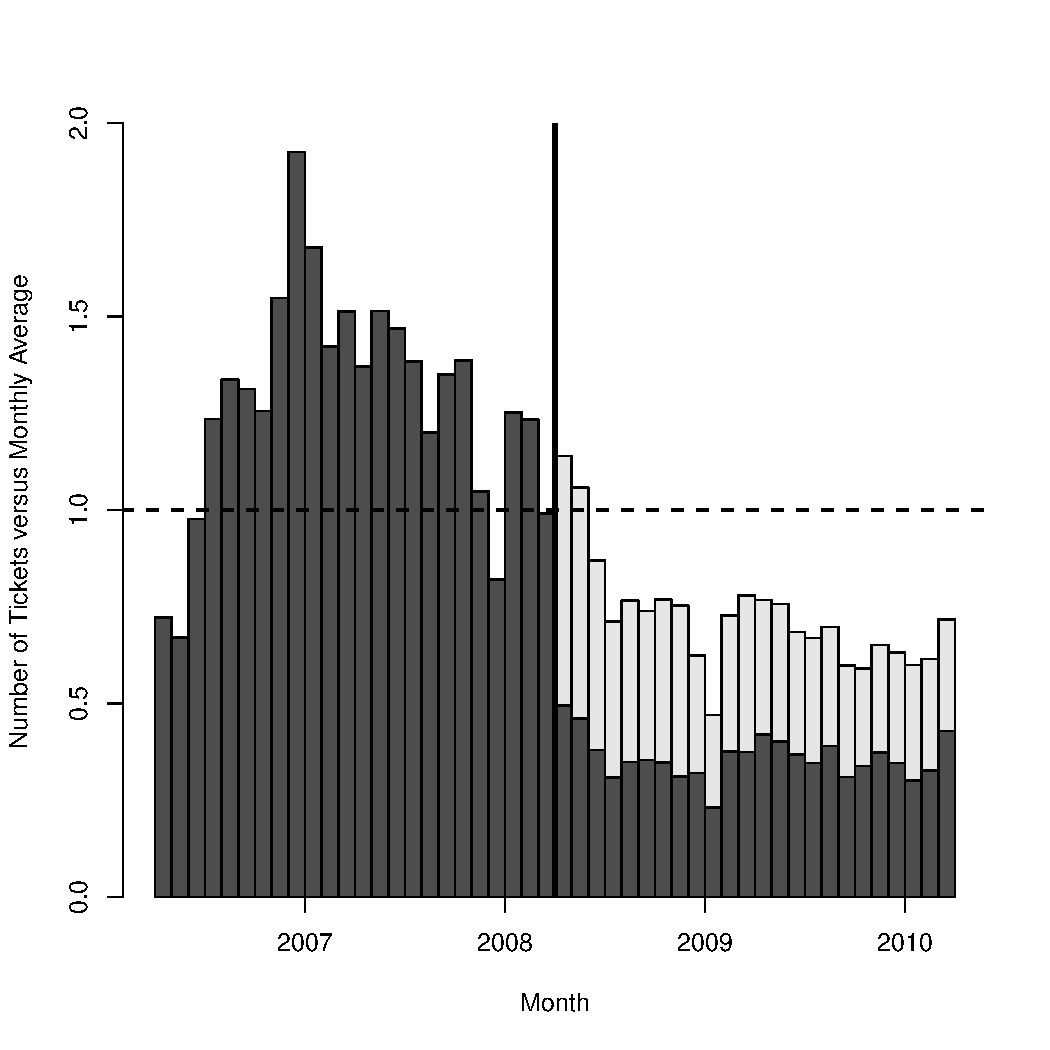
\includegraphics[width=0.8\textwidth]{Figures/num_pts_5_10_all}
\caption{Monthly frequency of 5- and 10-point violations }
Notes: Authors' calculations. 
Monthly frequency of 5-point violations before the policy change 
and 5- or 10-point violations after the policy change, 
divided by the average number of 5- and 10-point violations
for each calendar month. 
% 
The dashed line at $1.0$ indicates the point at which 
the number of tickets is equal to the average for each month 
for tickets of the same point values over the entire sample.
% 
Dark grey areas correspond to 5 point-stops and light grey areas to 10-point stops.
\label{fig:num_pts_5_10_all}
\end{figure}


Taking into consideration the seasonality of speeding, we see 
in Figure \ref{fig:num_pts_5_10_all}
an important reduction in the number of 5- or 10-point tickets 
in the summer of 2008 compared to the preceding summer. 
Overall, there is a general downward trend in the number of tickets 
after the policy change compared to before the policy change, 
and the 5- and 10-point tickets after the change are approximately evenly split. 

With 7- or 14-point stops,
in Figure \ref{fig:num_pts_7_14_all}, 
we see a different picture: 
nearly all 7-point violations are worth 14 points after the policy change, 
while only a few 7-point violations remain. 
Since there is no violation worth 7 points after the policy change, 
all of the 7-point stops after the policy change are due to being pulled over 
for multiple violations totalling 7 points. 
Once again, we see a downward trend in the number of total violations. 


\begin{figure}
\centering
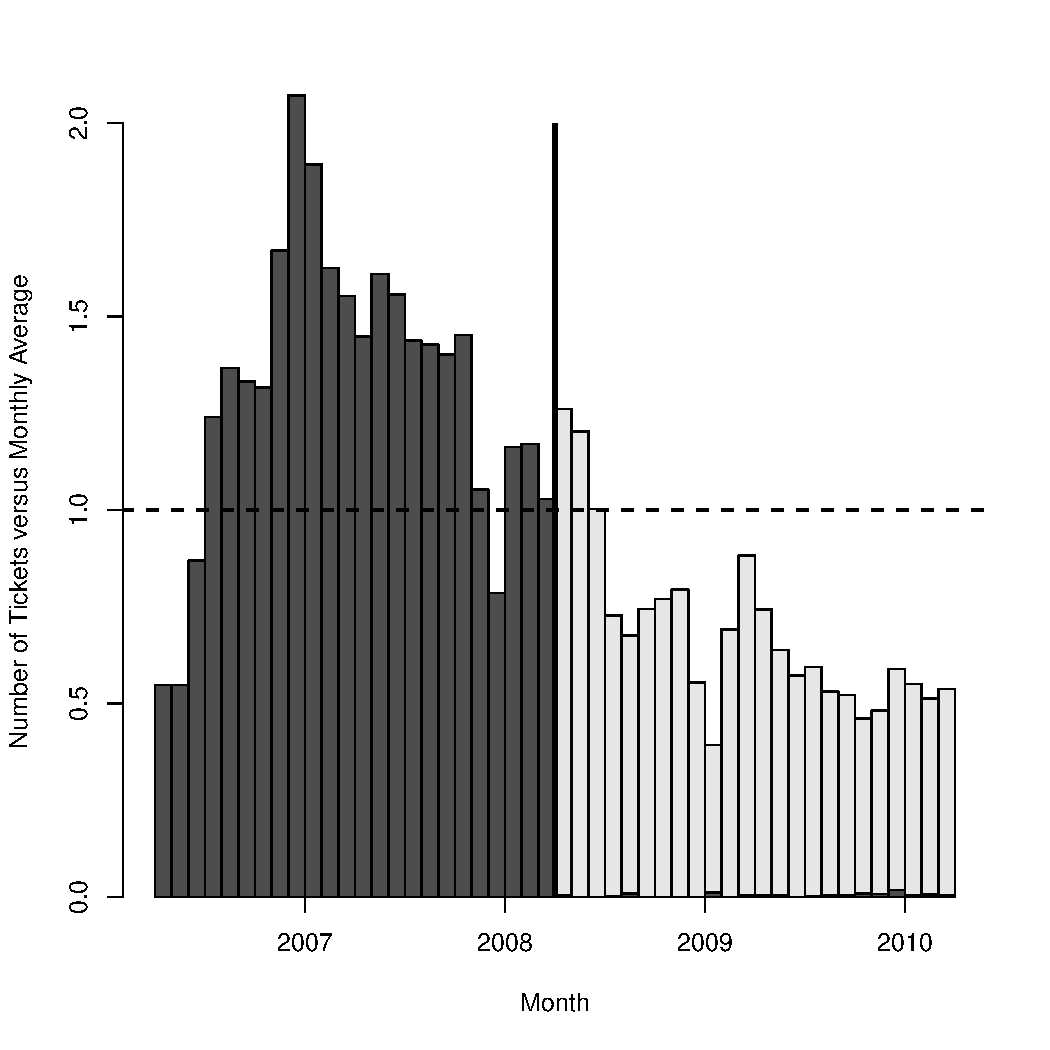
\includegraphics[width=0.8\textwidth]{Figures/num_pts_7_14_all}
\caption{Monthly frequency of 7- and 14-point violations }
Notes: Authors' calculations. 
Monthly frequency of 7-point violations before the policy change 
and 7- or 14-point violations after the policy change, 
divided by the average number of 7- and 14-point violations
for each calendar month. 
% 
The dashed line at $1.0$ indicates the point at which 
the number of tickets is equal to the average for each month 
for tickets of the same point values over the entire sample.
% 
Dark grey areas correspond to 7 point-stops and light grey areas to 14-point stops.
\label{fig:num_pts_7_14_all}
\end{figure}



\begin{table}% [ht]
\centering
\begin{tabular}{r r r r r r r}
  \hline
		& \multicolumn{2}{c}{Male Drivers} 	&  \multicolumn{2}{c}{Female Drivers} &  \multicolumn{2}{c}{Gender Ratio} \\
 & & & & & \multicolumn{2}{c}{(Percent Males)} \\

 \cmidrule(lr){2-3}\cmidrule(lr){4-5}\cmidrule(lr){6-7} 
%  \hline
Points 	& Pre 		& Post		& Pre 		& Post		& Pre 		& Post		\\ 
  \hline
1 		& 101,298 	& 122,899	&  45,382 	&   61,778 	& 69\% 	& 67\% \\ 
2 		& 533,167 	& 572,194	& 249,669 	& 283,108 	& 68\% 	& 67\% \\ 
3 		& 701,053 	& 627,807	& 247,991	& 239,554	& 74\% 	& 72\% \\ 
4 		&  15,567 	&  15,278 	&    2,216 	&    2,470 	& 88\% 	& 86\% \\ 
5 		&  43,006 	&  12,368 	&    8,172 	&    2,272 	& 84\% 	& 84\% \\ 
6 		&     496 	&  12,000 	&        21 	&    3,296 	& 96\% 	& 78\% \\ 
7 		&   7,688 	&        18 	&      648 	&          6 	& 92\% 	& 75\% \\ 
9 		&   7,382 	&    5,791 	&    2,587 	&    2,431 	& 74\% 	& 70\% \\ 
10 		&         0 	&  12,747 	&         0 	&    2,137 	& -			& 86\% \\ 
12 		&     127	&         0 	&         1 	&         0 	& 99\% 	& - \\ 
14 		&       0 	&   4,145 	&         0 	&      302 	& -			& 93\% \\ 
15 		&      17 	&         0 	&         1 	&         0 	& 94\% 	& - \\ 
18 		&       3 	&      560 	&         0 	&        23 	& 100\% 	& 96\% \\ 
24 		&       0 	&       98 	&         0 	&         4 	& -			& 96\% \\ 
30 		&       0 	&       17 	&         0 	&         0 	& -			& 100\% \\ 
36 		&       0 	&        4 	&         0 	&         0 	& -			& 100\% \\ 

   \hline

Total 	  & 1,409,804 & 1,385,926 & 556,688 & 597,381 & 72 & 70 \\ 

   \hline
\end{tabular}
\caption{Frequency of tickets by point value} 
The headings ``Pre'' and ``Post'' columns refer to offences that occurred before and after the policy change. 
The gender ratio is measured as the percentage of the number of offences committed by males 
divided by the total number of offences committed by all drivers. 
\label{tab:point_freq}
\end{table}

Table \ref{tab:point_freq} reports 
the number of tickets by point value, 
for male and female drivers, before and after the
change in penalties. 
%
In the 1- and 2-point categories, the number of tickets increases 
for both males and females on a per driver-day basis, 
and generally decreases in the higher-point categories. 
% 
Recall that several types of violations
earn a higher number of points after the policy change; 
for example, 
the 14-point tickets are all formerly 7-point tickets.

To put these numbers in a broader context, 
the vast majority of the sample are non-events. 
Before the excessive speeding law came into effect, 
the average driver had a probability of 0.04\% to receive a ticket 
on any particular day. 
This probability decreased by approximately 3.6\% after the policy change. 
If we look at the demerit points per driver per day, 
they decreased after the policy change for males by 6\% and by 1\% for females. 
This result is particularly interesting, 
because excessive speeding penalties doubled the value of many 
speeding violations previously worth 5, 7, and 9 points.\footnote{%  
Some 3-point speeding tickets are subject to the excessive speeding law, 
but the circumstances are quite particular: 
the suspect needs to be exceeding the speed limit in a zone 
with a posted limit of 60km/h or less by 40 to 45 km/h.}
In the absence of a change in behaviour, 
the number of demerit points per driver per day 
would have mechanically increased. 


Overall, females represent half of drivers 
yet only 20\% of all traffic tickets. 
%
The last two columns of
Table \ref{tab:point_freq}
report the gender ratio by point value.
% 
Females claim one third of the tickets for 1 or 2 points
but only a quarter of 3-point tickets. 
Males account for the majority of tickets with higher point values, 
with the gender ratio approaching 100\% male 
for the most severe cases of excessive speeding. 
% 
It might be the case that males drive more often than females; 
however, if that were the only cause of the difference, one would 
expect the gender ratio to be constant across the different point values. 
%
The extreme gender ratio in the upper tail for excessive speeding offences 
suggests that males engage in risky driving behaviour 
more often than females. 


% 
Economists
\citet{crosongneezy2009}
document a large literature 
analyzing gender differences in preferences from many perspectives, 
including financial decisions, as in
\citet{charnessgneezy2012}.   
% 
This topic has a long history in the psychological literature: 
\citet{byrnes1999}
reviewed
over 150 papers on gender differences in risk perception.
In their words, the literature ``clearly'' indicated that
``male participants are more likely to take risks than female
participants'' (p. 377). 
% 
Exploring factors aside from risk aversion, 
\citet{powellansic1997} report that the gender difference in risk-taking 
is irrespective of familiarity and framing, costs or ambiguity. 
% 
\citet{harris2006} 
consider not only the incidence and severity of
negative outcomes but also the enjoyment expected from 
engaging in risky activities. 
This 
partially mediated the perceived lower propensity of females
toward risky choices in decisions involving gambling, recreation, and health. 
We explore these differences in perception to explain 
the differences in both 
the tendency for speeding and 
the reaction when the cost of speeding increases. 


Aside from gender differences, 
there also exists the potential for differences by age, 
which is also observed in our dataset. 
%
In fact, this is also one of the main findings in 
\citet{byrnes1999}: 
there were significant shifts in the size of the gender gap between successive age levels.
% 
We explore this further with a more precise empirical specification. 


